\chapter{Theoretical and experimental basics}
\label{theory}

\section{The Standard Model of Particle Physics}

The Standard Model of Particle Physics summarizes the current knowledge of fundamental particles and their interactions. The model holds at scales of 1 fm and below. Gravity, being the fourth fundamental force is not included because it is negligible for most phenomena at this scale.
The current view is that all matter is made out of three kinds of elementary particle being leptons quarks and mediators.
There are six leptons falling into three families according to charge, electron number, muon number and tau number. To each of these leptons there also is an antilepton with all signs reversed.
Similiar to that there are six flavors of quarks separated by Strangeness (S), charm (C), Beauty (B), and truth (T). As well as the leptons the quarks fall into three generations.


\begin{table}[]
\centering
\caption{My caption}
\label{my-label}
\begin{tabular}{l|l|l|l|l|l|}
\cline{2-6}
                                   & symbol        & Charge $Q$ & $L_e$ & $L_{\mu}$ & $L_{\tau}$ \\ \cline{2-6} 
\multirow{2}{*}{First generation\{}  & $e$             & -1       & 1    & 0          & 0           \\ \cline{2-6} 
                                   & $\nu_e$        & 0        & 1    & 0          & 0           \\ \cline{2-6} 
\multirow{2}{*}{Second generation\{} & $\mu$           & -1       & 0    & 1          & 0           \\ \cline{2-6} 
                                   & $\nu_{\mu}$  & 0        & 0    & 1          & 0           \\ \cline{2-6} 
\multirow{2}{*}{Third generation\{}  & $\tau$          & -1       & 0    & 0          & 1           \\ \cline{2-6} 
                                   & $\nu_{\tau}$ & 0        & 0    & 0          & 1           \\ \cline{2-6} 
\end{tabular}
\end{table}

\begin{table}[]
\centering
\caption{My caption}
\label{my-label}
\begin{tabular}{l|l|l|l|l|l|l|l|l|}
\cline{2-9}
                                      & Symbol & Charge Q       & D  & U & S  & C & B  & T \\ \cline{2-9} 
\multirow{2}{*}{First generation \{}  & $d$    & $-\frac{1}{3}$ & -1 & 0 & 0  & 0 & 0  & 0 \\ \cline{2-9} 
                                      & $u$    & $\frac{2}{3}$  & 0  & 1 & 0  & 0 & 0  & 0 \\ \cline{2-9} 
\multirow{2}{*}{Second generation \{} & $s$    & $-\frac{1}{3}$ & 0  & 0 & -1 & 0 & 0  & 0 \\ \cline{2-9} 
                                      & $c$    & $\frac{2}{3}$  & 0  & 0 & 0  & 1 & 0  & 0 \\ \cline{2-9} 
\multirow{2}{*}{Third generation \{}  & $b$    & $-\frac{1}{3}$ & 0  & 0 & 0  & 0 & -1 & 0 \\ \cline{2-9} 
                                      & $t$    & $\frac{2}{3}$  & 0  & 0 & 0  & 0 & 0  & 1 \\ \cline{2-9} 
\end{tabular}
\end{table}





\section{The LHC and ATLAS}

The analysis for this thesis has been performed in the ATLAS collaboration. The ATLAS-Detector is one of the four big experiments at the LHC at Cern. Therefore this chapter gives a brief overview over the LHC and ATLAS focusing on the properties directly relevant for Particle Flow Analysis.

\subsection{The LHC}

The Large Hadron Collider ("LHC") at CERN was built to extend the frontiers of modern particle physics by delivering high luminosities and unprecedented high energies.\\
The LHC is designed to collide bunches of up to \num{d11} protons
\begin{figure}[htbp]
  \centering
  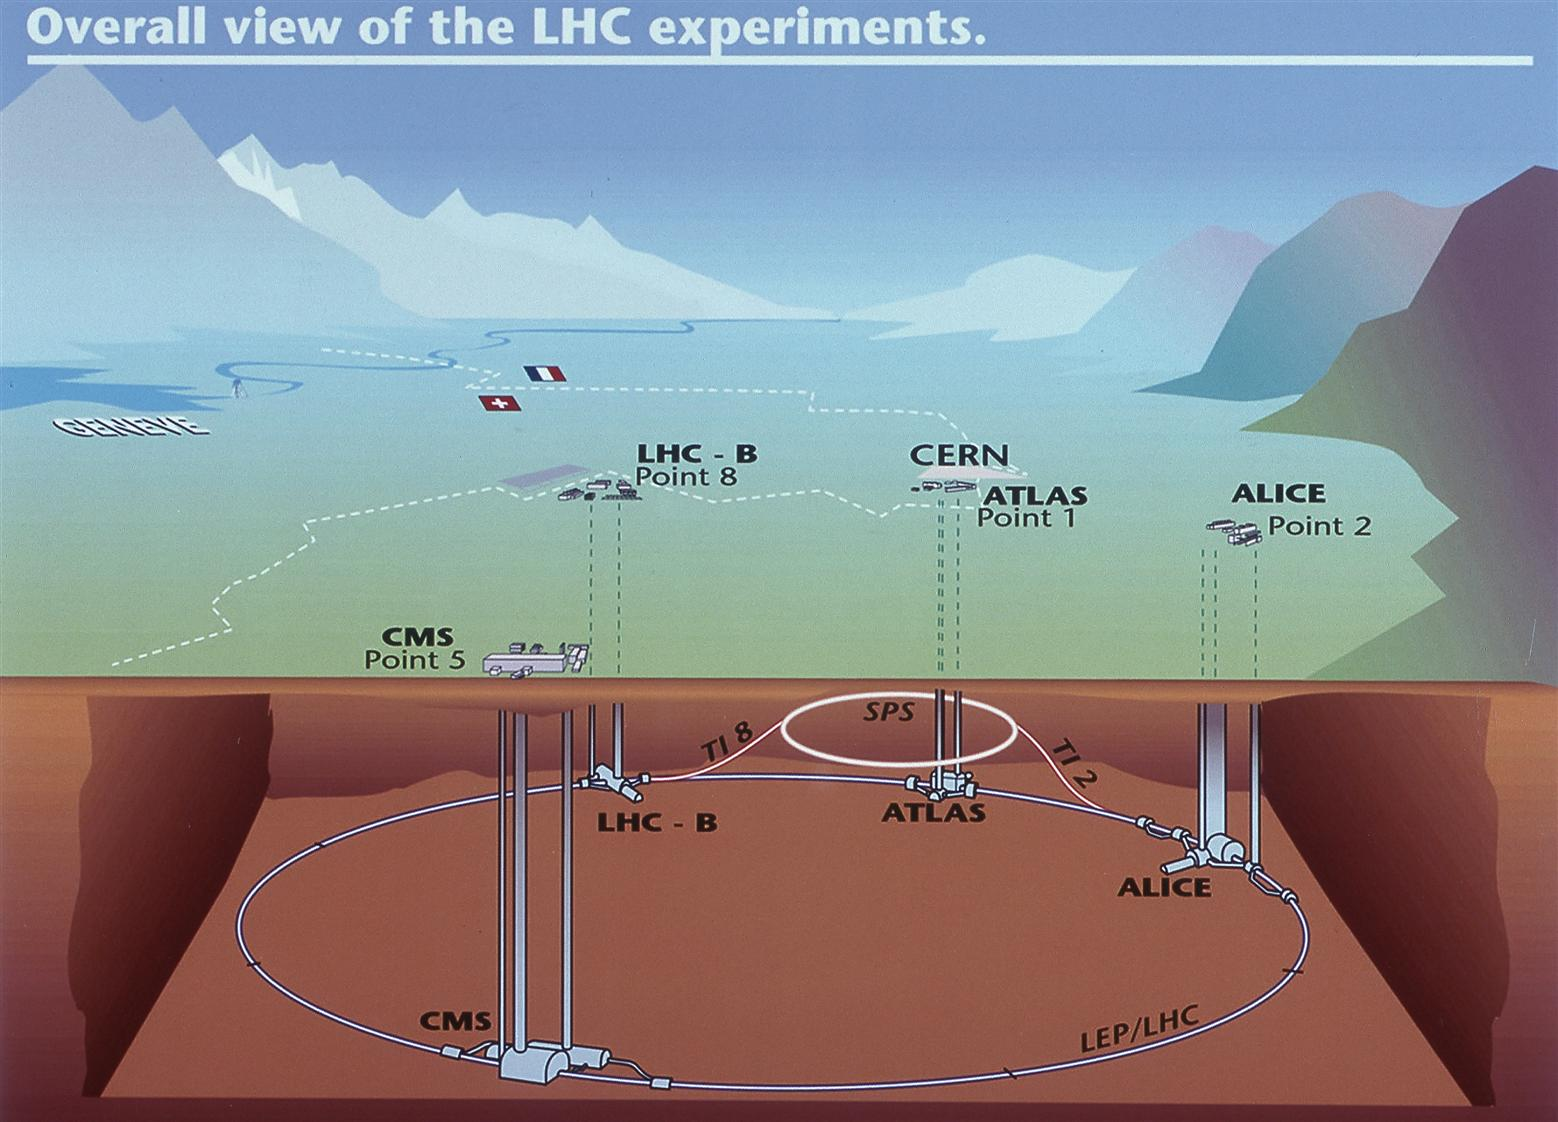
\includegraphics[width=\figwidth]{CERN_all-experiments}
  \caption[Sketch of the LHC ring, the position of the experiments and
  the surrounding countryside.]{Sketch of the LHC ring, the position
    of the experiments and the surrounding countryside. The four big
    LHC experiments are indicated. The location of the injection lines
    and the SPS are also shown.}
  \label{fig:LHC}
\end{figure}


\subsection{The ATLAS Detector}

\begin{figure}[htbp]
  \centering
  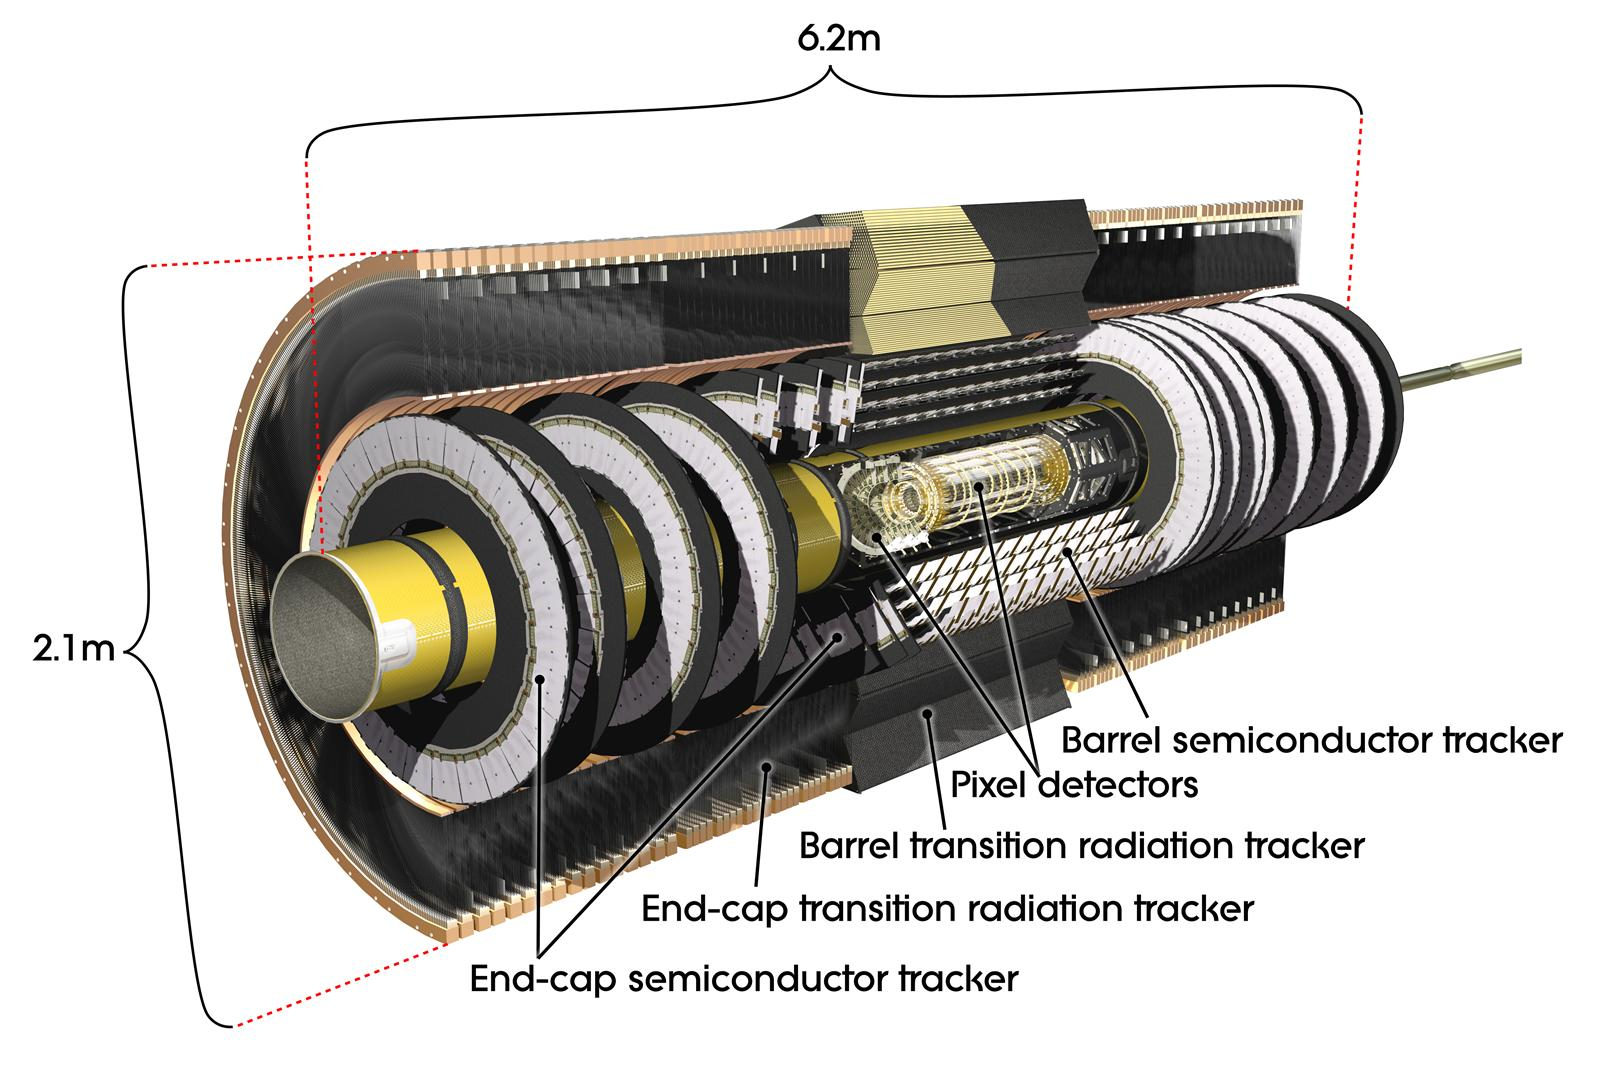
\includegraphics[width=\figwidth]{atlas-detector}
  \caption[Sketch of the LHC ring, the position of the experiments and
  the surrounding countryside.]{Sketch of the ATLAS detector}
  \label{fig:atlas}
\end{figure}




\section{The Particle Flow Algorithm}

Recently only either the Calorimeter or the tracker information was used to reconstruct Jets in ATLAS events. The Particle Flow Algorithm combines tracker and calorimeter information to achieve better resolution especially at lower energies. The main advantages of including the tracker information into reconstruction are listed here:


\begin{itemize}
\item For low energy charged particles the momentum resolution of the tracking detector is superior to the calorimeter.
\item The Tracking detector is able to reconstruct softe particles, which would not pass the noise threshold of the calorimeter.
\item The ATLAS traking detector has a superior angular resolution for single charged particles.
\item Low $p_T$ charged particles may be swept out of the cone before reaching the calorimeter by the magnetic field. The tracker information allows to cluster these particles into the jet.
\end{itemize}


\section{Calibration in Particle Flow and its difficulties at the time}